\appendix


\begin{center}
  \Large\textbf{Appendix}
\end{center}

\section{Clinical Thresholds for Target Complications}
\label{app:clinical-thresholds}

To obtain precise event times, all target complications are defined directly from physiological measurements rather than diagnosis codes. The six outcomes predicted during the 48--336\,h prediction window are defined by the following clinical thresholds applied directly to raw MIMIC-IV laboratory values:

\begin{itemize}
    \item \textbf{Hyperglycemia:} A glucose measurement $\ge$ 250 mg/dL, OR a glucose measurement $\ge$ 180 mg/dL with a prior glucose measurement also $\ge$ 180 mg/dL (recurrent).
    \item \textbf{Severe Hyperglycemia:} A single glucose measurement $\ge$ 250 mg/dL.
    \item \textbf{Hypoglycemia:} A glucose measurement $\le$ 54 mg/dL, OR a glucose measurement $\le$ 70 mg/dL with a prior measurement between 20 and 70 mg/dL (recurrent).
    \item \textbf{Severe Hypoglycemia:} A single glucose measurement $\le$ 54 mg/dL.
    \item \textbf{Kidney Complication (Acute Kidney Injury):} A serum creatinine measurement $\ge$ 4.0 mg/dL (AKI Stage 3 criterion), OR a serum creatinine measurement that is $\ge$ 2.0 times the baseline creatinine measurement recorded at admission (AKI Stage 2+ criterion).
    \item \textbf{Death:} Defined by the patient's recorded time of death. To capture all relevant critical care mortality, this includes hospital mortality as well as 30-day post-discharge mortality where linked via state death records.
\end{itemize}

By deriving outcome labels from timestamped physiological measurements whenever possible, the prediction task requires forecasting clinically meaningful deterioration rather than recovering broad administrative diagnoses.

\section{Architectural Ablation Trail}
\label{app:ablation-trail}

The architectures reported in the main paper are the endpoints of an iterative design search documented here. Early experiments were conducted on a 10k-admission design subset to explore architectural choices, followed by confirmation on the full training cohort using the final recipes. Intermediate design stages report only the metrics tracked during the corresponding search and therefore contain ``--'' where metrics were not evaluated.

\subsection{Decoder ablations}

% --- Decoder: consolidated architectural trail (single table) ---
\begin{table*}[h]
\caption{INTERVenE-Ar architectural trail, stratified by sample size. Reading order: foundational 10k build-up; 10k component-drop ablations of the locked recipe; full-cohort build-up to the deployed recipe. \texttt{-} = not measured at that design stage. Intermediate rows reflect the configuration \emph{as it stood} at each design point, not the deployed recipe with one component removed. Full-cohort: 95\% bootstrap CI half-widths (2{,}000-resample); 10k: point estimates. \emph{gen/GT}: median generated/ground-truth length ratio.}
\label{tab:abl-ar-all}
\centering
\small
\setlength{\tabcolsep}{4pt}
\begin{tabular}{llcccc}
\toprule
Recipe arm & Sample & AUROC$_w$ & AUPRC$_w$ & LoS MAE (h) & gen/GT \\
\midrule
Baseline decoder (no TTT aux / pool / gate)      & 10k  & $0.836$                    & $0.539$                    & -                       & $0.60$ \\
\quad + TTT aux head + TTT-guided inference      & 10k  & $0.840$                    & $0.542$                    & -                       & $0.72$ \\
\midrule
\textbf{Locked recipe (10k retrain, anchor)} $=$ \textbf{above} $+$ \textbf{patient-pool aux}     & 10k  & $\mathbf{0.845}$           & $\mathbf{0.562}$           & $71.3$                  & $0.44$ \\
\quad $-$ Phase-3 finetune (eval-only on P2)     & 10k  & $0.547$                    & $0.213$                    & $67.8$                  & $0.66$ \\
\quad $-$ RoPE                                   & 10k  & $0.830$                    & $0.525$                    & $98.3$                  & $1.79$ \\
\quad $-$ CBM                                    & 10k  & $0.834$                    & $0.534$                    & $71.0$                  & $1.09$ \\
\quad $-$ soft kernel ($\tau{=}0.5$\,h)          & 10k  & $0.808$                    & $0.500$                    & $111.7$                 & $2.16$ \\
\quad DD damping $\sqrt{}$                       & 10k  & $0.801$                    & $0.493$                    & $69.6$                  & $1.16$ \\
\quad DD damping $\log$ (under-correct)          & 10k  & $0.797$                    & $0.503$                    & $95.7$                  & $1.79$ \\
\midrule
Prior canonical (ttt cap $0.30$, no DD weighting)       & full & $0.832{\pm}0.007$          & $0.519{\pm}0.015$          & $147.7{\pm}1.9$         & $2.82$ \\
\quad + ttt cap $0.30{\to}0.60$            & full & $0.832{\pm}0.007$          & $0.562{\pm}0.013$          & $78.7{\pm}1.0$          & $1.06$ \\
\quad + DD-$p^{0.33}$ weighting \textbf{= Ar-final (deployed)} & full & $\mathbf{0.854{\pm}0.007}$ & $\mathbf{0.587{\pm}0.013}$ & $\mathbf{65.1{\pm}1.1}$ & $\mathbf{0.90}$ \\
\bottomrule
\end{tabular}
\end{table*}

\textbf{Decoder trail (Table~\ref{tab:abl-ar-all}).}
The 10k design search established the core decoder recipe: the \texttt{ttt} auxiliary head improved trajectory-end anticipation, the patient-pool auxiliary provided the largest discrimination gain, and the \texttt{ttt} inference gate restored realistic trajectory lengths at evaluation time. Component-drop ablations identify Phase-3 fine-tuning as the dominant contributor, while RoPE, CBM, the soft-kernel loss, and the damping function each make measurable contributions to trajectory quality and predictive performance. Full-cohort confirmation shows that the deployed recipe substantially improves discrimination, trajectory fidelity (gen/GT), and LoS prediction over the prior canonical implementation. \textbf{DD-$p^{0.33}$ weighting} applies the per-terminal-token class-imbalance ratio (neg/pos) raised to the power $0.33$ as the LM-head BCE positive weight. Compared with $\sqrt{\cdot}$ and $\log$ damping, it provides the best compromise between over- and under-generation, restoring realistic trajectory lengths while preserving predictive performance.

\subsection{Encoder ablations}

INTERVenE-Enc builds directly on the decoder backbone, inheriting the architectural components validated in Table~\ref{tab:abl-ar-all} (hierarchical token embeddings, Time2Vec, temporal RoPE, AdaLN-Zero conditioning, the per-outcome attention pool, and the soft-kernel BCE). These components are therefore held fixed; the encoder ablations isolate only the additions specific to the bidirectional setting: Phase-3 risk--time loss balancing, Phase-3 backbone learning, the forward-addition trail of inverse-prevalence weighting, focal loss and CBM masking, and the input-representation alternative.

% --- Encoder: consolidated architectural trail (single table) ---
\begin{table*}[h]
\caption{INTERVenE-Enc architectural trail, stratified by sample size. Reading order: 10k design search; 10k ablation of the locked recipe; full-cohort build-up to the deployed recipe plus one input-representation alternative. \texttt{-} = not measured at that design stage. CI and intermediate-row conventions as in Table~\ref{tab:abl-ar-all}.}
\label{tab:abl-enc-all}
\centering
\resizebox{\textwidth}{!}{%
\begin{tabular}{llccc}
\toprule
Recipe arm & Sample & AUROC$_w$ & AUPRC$_w$ & LoS MAE (h) \\
\midrule
\textbf{Locked recipe (10k retrain, anchor)}             & 10k  & $\mathbf{0.822}$  & $\mathbf{0.497}$  & $53.0 \pm 2.1$ \\
\quad + hierarchical MLM masking                         & 10k  & $0.820$           & $0.482$           & - \\
\quad + backbone LR factor $0.01 \to 0.1$                & 10k  & $0.813$           & $0.471$           & - \\
\quad $-$ Phase-3 backbone learning$^\dagger$            & 10k  & $0.792$           & $0.429$           & $55.3 \pm 2.3$ \\
\midrule
Stripped baseline (full data, KBTA input)                & full & $0.901 \pm 0.005$ & $0.662 \pm 0.013$ & $46.1 \pm 0.9$ \\
\quad + inverse-prevalence pos-weight$^\dagger$          & full & $0.894 \pm 0.005$ & $0.638 \pm 0.013$ & $49.1 \pm 0.8$ \\
\quad + focal loss, $\gamma{=}1.0$                       & full & $0.901 \pm 0.005$ & $0.665 \pm 0.012$ & $44.7 \pm 0.8$ \\
\quad + CBM masking $p{=}0.15$ \textbf{= Enc-final (deployed)} & full & $\mathbf{0.901 \pm 0.005}$ & $\mathbf{0.672 \pm 0.012}$ & $\mathbf{44.4 \pm 0.9}$ \\
\midrule
Enc-final with std-bins input (KBTA replaced)            & full & $0.901 \pm 0.005$ & $0.676 \pm 0.012$ & $47.6 \pm 0.9$ \\
Enc-final with de-intervaled input & full & $0.864 \pm 0.007$ & $0.593 \pm 0.015$ & $51.8 \pm 0.8$ \\
\bottomrule
\end{tabular}%
}

\smallskip
\footnotesize $^\dagger$Non-overlapping bootstrap CIs vs.\ the 10k anchor (backbone freeze) or vs.\ the stripped baseline (inv-prev weighting). Focal loss and std-bins rows are within CI noise on AUPRC/AUROC; std-bins LoS $+3.2$\,h is non-overlapping. Hierarchical MLM masking and backbone-LR rows were discarded after 10k search.
\end{table*}

\textbf{Encoder trail (Table~\ref{tab:abl-enc-all}).}
The 10k design search established the Phase-3 training recipe, showing that reducing the time-loss weight substantially improves discrimination while hierarchical MLM masking provides no measurable benefit. Component-drop ablations identify Phase-3 backbone learning as essential, whereas the full-cohort study shows that inverse-prevalence weighting degrades performance, focal loss has negligible effect, and CBM masking ($p{=}0.15$) provides the only consistent improvement over the stripped baseline. Finally, replacing KBTA with a standard-deviation discretization preserves AUPRC and AUROC but increases LoS error, supporting the use of KBTA for interpretability while retaining a modest regression advantage. Crucially, collapsing the intervals into 1-second point events sharply degrades performance across all metrics (weighted AUPRC dropping to $0.593$), demonstrating that the architecture explicitly relies on capturing continuous temporal durations and state concurrency rather than acting as a simple point-event detector.

% --- Encoder: capacity + heads (sweet-spot table) ---
\begin{table*}[h]
\caption{INTERVenE-Enc capacity and head-count ablations (full cohort, locked recipe except the dimension under test). Bold = deployed M-128/h=2 configuration. CI conventions as in Table~\ref{tab:abl-ar-all}; size-sweep arms predated LoS tracking (\texttt{-}).}
\label{tab:abl-enc-capacity}
\centering
\small
\setlength{\tabcolsep}{4pt}
\begin{tabular}{lccccccc}
\toprule
Variant & embed\_dim & n\_head & head\_dim & Params & AUPRC$_w$ & AUROC$_w$ & LoS MAE (h) \\
\midrule
M-64                                  & 64   & 1 & 64 & 0.46M & $0.646$                    & $0.889$                    & -                       \\
\textbf{M-128 (Enc-final, deployed)}  & 128  & 2 & 64 & 1.84M & $\mathbf{0.672 \pm 0.012}$ & $\mathbf{0.901 \pm 0.005}$ & $\mathbf{44.4 \pm 0.9}$ \\
M-256                                 & 256  & 4 & 64 & 6.40M & $0.650$                    & $0.895$                    & -                       \\
\midrule
h=8 narrow heads (budget-preserving)  & 128  & 8 & 16 & 1.84M & $0.659 \pm 0.013$          & $0.900 \pm 0.005$          & $46.6 \pm 0.9$          \\
h=8 wide heads (parameter-spending)   & 512  & 8 & 64 & 25.0M & $0.676 \pm 0.012$          & $0.905 \pm 0.005$          & $45.2 \pm 0.9$          \\
\bottomrule
\end{tabular}
\end{table*}

\textbf{Capacity and heads (Table~\ref{tab:abl-enc-capacity}).} Model capacity exhibits a clear inverted-U, with the deployed M-128 configuration providing the best accuracy--efficiency trade-off. Increasing model width or attention-head count beyond this point yields little additional predictive benefit despite substantially larger parameter budgets, while smaller models underfit. Notably, even the M-64 configuration outperforms the strongest neural baseline (ss-STraTS), indicating that the headline improvements are driven primarily by the architecture rather than model capacity.

\textbf{STraTS dimensional shape.} INTERVenE-Enc is not evaluated at STraTS's deployed shape (dim=64, h=16, head\_dim=4, $\sim$86K parameters): M-64 underfits and narrow heads at dim=128 both cost AUPRC and LoS, so combining them would compound both losses. The intended comparison is each model at its own tuned configuration.

\section{Calibration}
\label{app:calibration}

Calibration is evaluated without retraining: locked checkpoints remain unchanged, and only the test-time logit-to-probability mapping is optimized.

\subsection{INTERVenE-Enc}

Per-outcome temperatures $T_k$ are fit by LBFGS on the validation split and applied unchanged to the held-out test split. Rank-based metrics are unaffected by the monotonic scaling.

\begin{table}[h]
  \caption{Enc per-outcome $T_k$ (validation fit) and ECE before/after scaling (test split). $T_k{=}1$ = perfectly calibrated; $T_k{>}1$ = over-confident. Last row: support-weighted aggregate.}
  \label{tab:calibration}
  \centering
  \resizebox{\columnwidth}{!}{%
  \begin{tabular}{lcccc}
    \toprule
    Outcome & $T_k$ & ECE$_\text{uncal}$ & ECE$_\text{cal}$ & $\Delta$ECE \\
    \midrule
    KIDNEY                  & 0.866 & 0.0228 & 0.0151 & $-0.0077$ \\
    SEVERE\_HYPERGLYCEMIA   & 0.907 & 0.0224 & 0.0176 & $-0.0048$ \\
    SEVERE\_HYPOGLYCEMIA    & 0.913 & 0.0101 & 0.0067 & $-0.0033$ \\
    HYPERGLYCEMIA           & 0.970 & 0.0166 & 0.0157 & $-0.0010$ \\
    HYPOGLYCEMIA            & 0.974 & 0.0071 & 0.0080 & $+0.0009$ \\
    DEATH                   & 1.039 & 0.0097 & 0.0075 & $-0.0022$ \\
    \midrule
    Weighted (by $n_\text{pos}$) & --- & $0.0162$ & $0.0134$ & $-0.0027$ \\
    \bottomrule
  \end{tabular}%
  }
\end{table}

\textbf{Findings.}
INTERVenE-Enc is well calibrated as emitted, with temperatures close to unity ($T_k\in[0.87,1.04]$). Temperature scaling yields only a modest improvement in support-weighted ECE ($0.016\rightarrow0.013$), consistent with the reliability diagrams (Figure~\ref{fig:reliability}). We nevertheless provide the fitted temperatures alongside the released checkpoint as an optional refinement.

\begin{figure*}[!t]
  \centering
  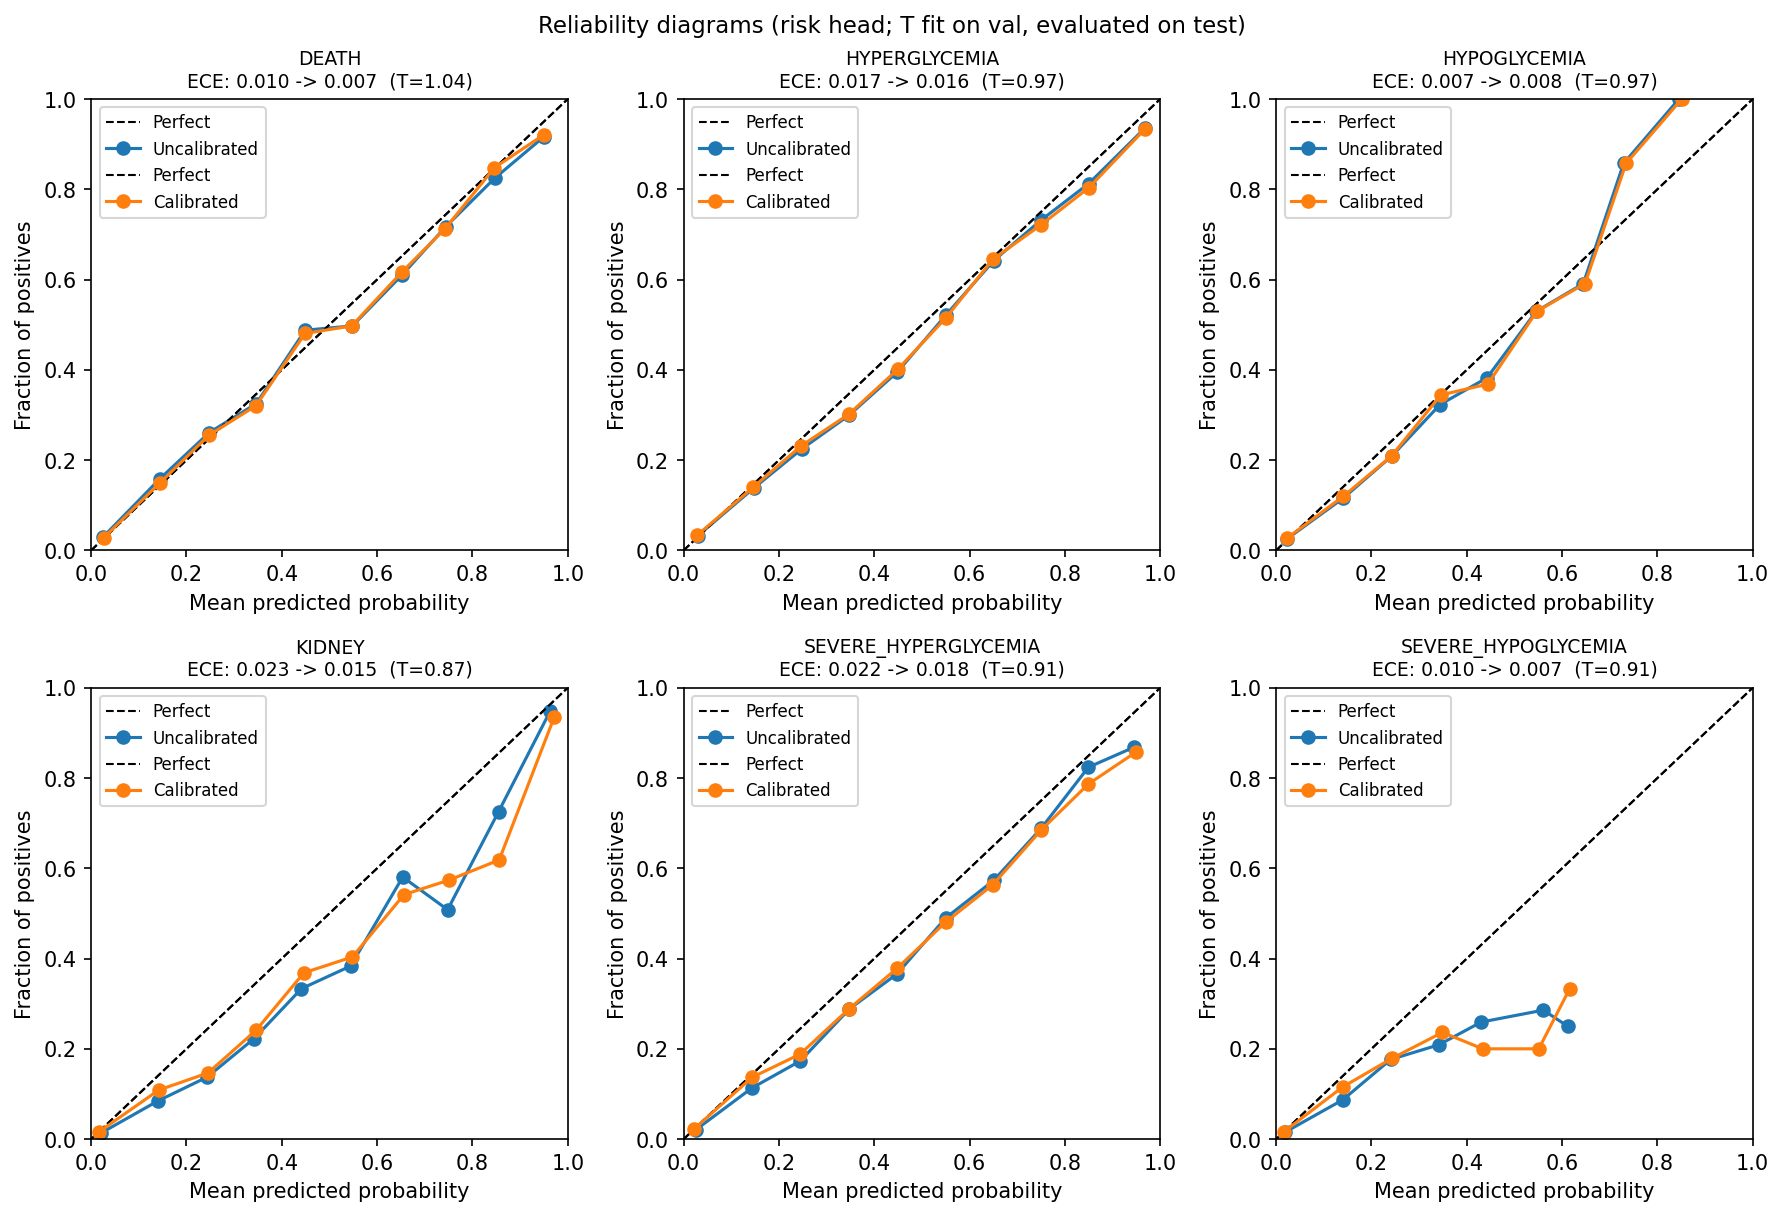
\includegraphics[width=\textwidth]{enc_reliability.png}
  \caption{INTERVenE-Enc reliability diagrams (10 equi-width bins, held-out test split). Blue: uncalibrated; orange: after $T_k$ scaling. Dashed diagonal = perfect calibration. Panel titles report ECE and $T_k$.}
  \label{fig:reliability}
\end{figure*}

\subsection{INTERVenE-Ar}

Calibration follows the same protocol, using the per-patient maximum outcome probability over the generated trajectory (the same readout used for the headline metrics). Temperatures are fit on the validation split and applied unchanged to the held-out test split.

\begin{table}[h]
  \caption{Ar per-outcome $T_k$ (validation fit) and ECE before/after scaling (test split). $T_k{<}1$ = over-confident; $T_k{>}1$ = under-confident. Readout: per-patient max $P_\text{outcome}$ over generated positions.}
  \label{tab:ar-calibration}
  \centering
  \resizebox{\columnwidth}{!}{%
  \begin{tabular}{lcccc}
    \toprule
    Outcome & $T_k$ & ECE$_\text{uncal}$ & ECE$_\text{cal}$ & $\Delta$ECE \\
    \midrule
    SEVERE\_HYPOGLYCEMIA    & 0.6543 & 0.1119 & 0.0754 & $-0.0365$ \\
    HYPOGLYCEMIA            & 0.7838 & 0.1174 & 0.0911 & $-0.0263$ \\
    KIDNEY                  & 0.9566 & 0.0523 & 0.0490 & $-0.0033$ \\
    SEVERE\_HYPERGLYCEMIA   & 1.0241 & 0.0450 & 0.0469 & $+0.0018$ \\
    HYPERGLYCEMIA           & 1.2365 & 0.0389 & 0.0184 & $-0.0205$ \\
    DEATH                   & 1.4700 & 0.0495 & 0.0108 & $-0.0387$ \\
    \bottomrule
  \end{tabular}%
  }
\end{table}

\textbf{Findings (Ar).}
INTERVenE-Ar exhibits a wider range of fitted temperatures than the encoder ($T_k\in[0.65,1.47]$), reflecting the greater calibration challenge of the autoregressive readout. Temperature scaling substantially improves calibration on the prevalent outcomes (e.g., DEATH: $0.050\rightarrow0.011$ ECE), while the rare hypoglycemia outcomes remain the most difficult to calibrate, consistent with their low prevalence and AUPRC. Reliability diagrams are shown in Figure~\ref{fig:ar-reliability}; fitted temperatures are supplied alongside the checkpoint. Aggregate ECE is omitted because calibration is evaluated on the trajectory-derived peak-probability readout rather than a native discriminative output.

\begin{figure*}[!t]
  \centering
  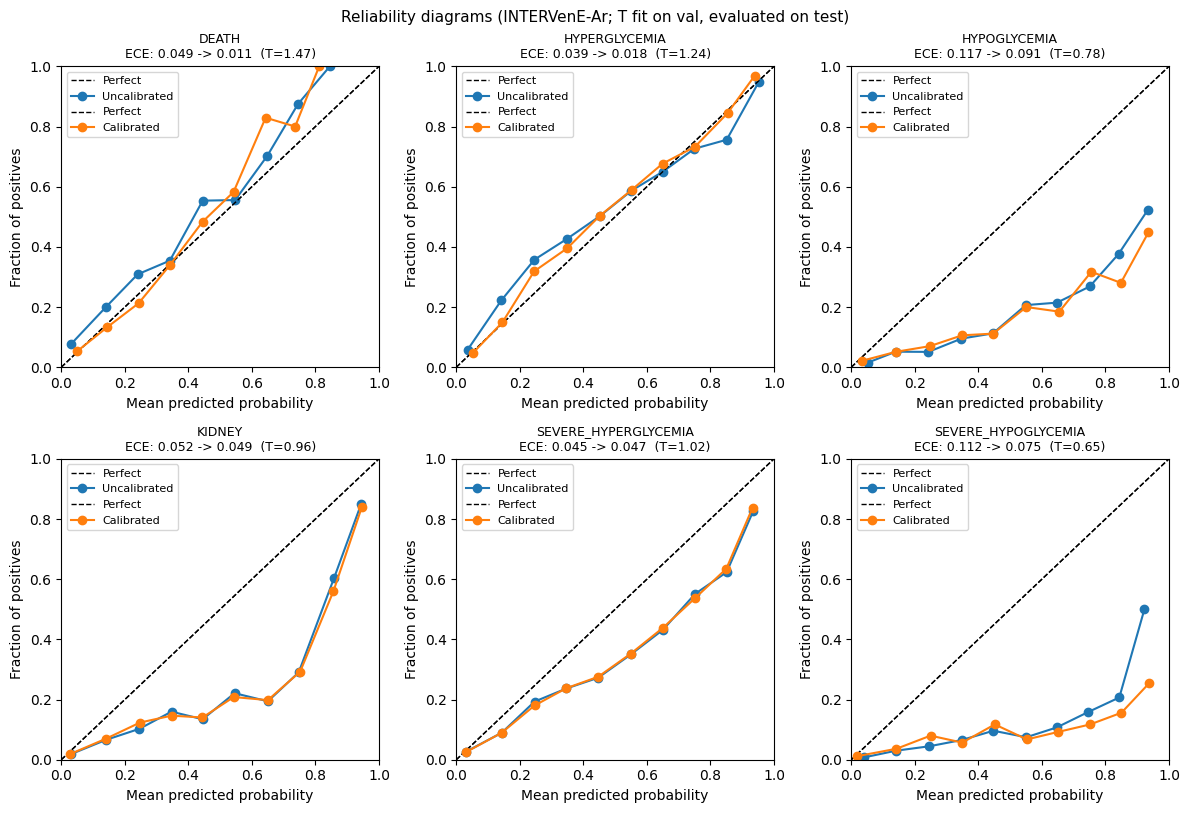
\includegraphics[width=\textwidth]{ar_reliability.png}
  \caption{INTERVenE-Ar reliability diagrams (10 equi-width bins, held-out test split). Blue: uncalibrated; orange: after $T_k$ scaling. Prevalent outcomes improve substantially after scaling (DEATH $0.050\!\to\!0.011$); rare hypoglycaemia panels show wider residual deviation consistent with the AUPRC floor in the per-outcome retults table in the main paper.}
  \label{fig:ar-reliability}
\end{figure*}

\section{Autoregressive Risk Trajectories}
\label{app:ar-trajectories}
The Ar variant emits a per-step risk curve over the generated trajectory. The risk head is evaluated at every generation step, producing a time-resolved signal that can express multiple risk peaks within an admission. Peak width is governed by the Phase-2 soft-kernel ($\tau=12$\,h for DEATH); absolute risk values should therefore be interpreted relative to $\tau$ rather than as binary decisions. Figure~\ref{fig:ar-trajectory} illustrates two representative test patients.

\begin{figure}[!t]
  \centering
  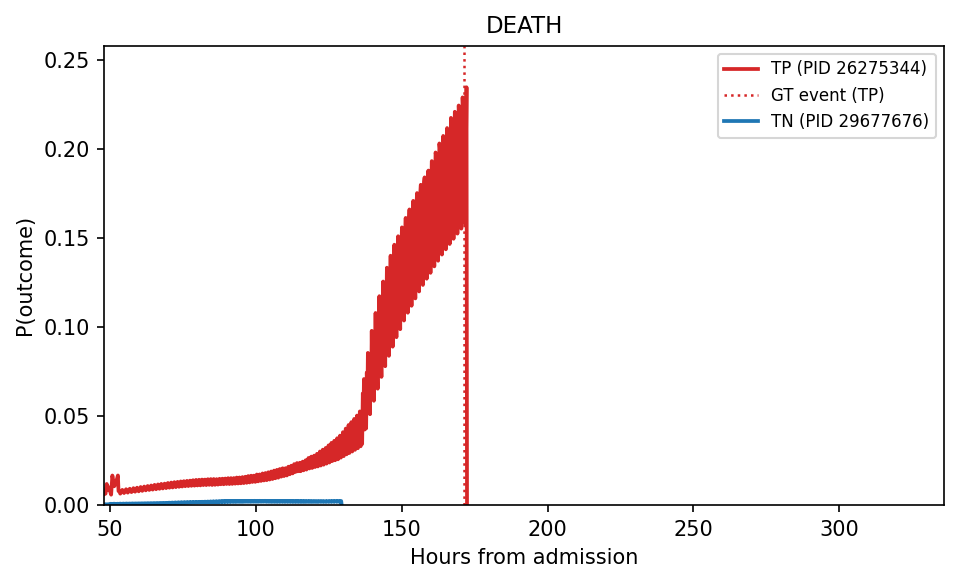
\includegraphics[width=\columnwidth]{ar_risk_trajectory_death.png}
  \caption{INTERVenE-Ar per-step DEATH risk trajectories for two held-out test patients. Red: a true-positive admission, where risk progressively increases and peaks near the recorded death time ($\approx171$\,h, dotted). Blue: a true-negative admission, where risk remains near baseline throughout the generated trajectory. The $x$-axis begins at the 48\,h observation cutoff; the $y$-axis is normalized to the local peak.}
  \label{fig:ar-trajectory}
\end{figure}

\section{Implementation Details}
\label{app:implementation}

\paragraph{Computing infrastructure.}
Both INTERVenE variants were trained on a single NVIDIA RTX~A5000 (24\,GB VRAM) using PyTorch 2.4.1+cu124, CUDA 12.4 (cuDNN 9.1.0), and Python 3.11. All experiments use a fixed random seed of 42. The full pipeline (all three phases) runs without multi-GPU or distributed training.

\paragraph{Optimizer and regularization.}
All phases use AdamW with weight decay $0.001$ and gradient clipping at $\mathrm{max\_norm}{=}1.0$ applied at every update step. Betas differ by phase: Phase~1 (embedder pre-training in both variants) and INTERVenE-Ar Phase~3 use AdamW defaults $(0.9,\,0.999)$; INTERVenE-Enc Phases~2--3 and INTERVenE-Ar Phase~2 use $(0.9,\,0.95)$. The Phase~1 scheduler is ReduceLROnPlateau (factor $0.5$, patience $4$, min LR $10^{-6}$); Phases~2 and~3 use OneCycleLR.

\paragraph{Batch size and learning rates.}
The physical batch size is 16 with gradient accumulation over 4 steps (effective batch size 64). Phase~1 and Phase~2 use a peak LR of $3{\times}10^{-4}$; Phase~3 trains the task head at $10^{-4}$ with the backbone running at a fixed fraction ($0.1{\times}$ for INTERVenE-Enc, $0.01{\times}$ for INTERVenE-Ar). LR was selected from the range $[10^{-3},\,10^{-5}]$ based on validation loss behavior.

\paragraph{Legality masking (INTERVenE-Ar Phase 2).}
At each position $i$, a dynamic boolean mask $\mathbf{m}_i \in {0,1}^{V}$ is computed from the accumulated sequence state and applied to both the logits and the BCE targets, ensuring the model never receives gradient signal for illegal continuations. Illegality is determined by three stateful rules: (i) an interval \texttt{END} token is illegal if its corresponding \texttt{START} has not been seen; (ii) an interval \texttt{START} token is illegal if the same base or a conflicting value of the same concept is already open; (iii) meal tokens must follow a fixed cyclic order. The mask is derived deterministically from the TAK interval grammar at every training step and is recomputed autoregressively during generation.

\paragraph{Soft-kernel horizons and Phase 2 label exposure.}
The terminal BCE window is $H_\text{term}{=}168$\,h; the outcome risk-head horizon is $H_\text{out}{=}48$\,h (positive signal fires within 48\,h of an outcome event). Per-class decay $\tau_k$ is initialized at 48\,h for outcome tokens and 12\,h for terminal and default LM tokens; the terminal $\tau$ is frozen after an early diagnostic showed unconstrained widening, while the outcome $\tau$ remains learnable in Phases~2 and is frozen in Phase~3. Phase~2 pretraining trains on full patient trajectories and therefore sees post-48\,h tokens --- this is intentional, as the generative objective requires learning future sequence structure. Outcome labels (whether a complication occurs in hours 48--336) are introduced only in Phase~3; inference is seeded solely with the 0--48\,h input window, so no task-relevant label information is accessible during Phase~2 pretraining.

\paragraph{Auxiliary curriculum.}
Phases~2 and~3 apply a staged auxiliary unlock schedule: each auxiliary loss activates only after a minimum number of BCE-only warmup epochs and ramps to its configured fraction cap over a per-auxiliary ramp window. This governs the order and pace at which auxiliary losses become active --- it is a curriculum over loss composition, not a learning-rate warmup.

\paragraph{Early stopping and actual convergence.}
Each phase is capped at 100 epochs; training halts when the validation loss fails to improve by a minimum relative margin of $0.001$ for 10 consecutive epochs (patience searched over $5$--$15$). Actual convergence: both variants share the Phase~1 embedder, which ran 27 epochs (best checkpoint at epoch 22). INTERVenE-Enc Phase~2 ran 99 epochs (best at epoch 94); Phase~3 ran 49 epochs (best at epoch 44). INTERVenE-Ar Phase~2 ran 32 epochs (best at epoch 27); Phase~3 ran 70 epochs (best at epoch 65). The 2{,}000-resample patient-level bootstrap on the held-out test set serves as the per-metric uncertainty estimate in lieu of multi-seed retraining (see Limitations).

\paragraph{Generation horizon (INTERVenE-Ar).}
Autoregressive generation is bounded by two stopping criteria: a token budget of 2{,}000 and a temporal limit of 336 hours from admission. Generation also halts early upon emitting a terminal token (DEATH/RELEASE). In practice the temporal or terminal condition is binding; the token budget is a safety cap.

\section{Sparse-Transcoder Interpretability}
\label{app:xai}

This appendix expands the interpretability analysis summarized in the main text. We train one JumpReLU transcoder \citep{rajamanoharan2024jumping} per INTERVenE-Enc block on activations captured from a 1{,}500-patient stratified subset of the test cohort. Each transcoder reconstructs its block's MLP output from an overcomplete sparse dictionary (16$\times$ expansion; 2{,}048 features per layer). Reconstruction quality is high (per-layer $R^2=0.97$--$0.995$), while sparsity remains between approximately 5--19\% active features. The transcoders are used only for attribution and are never substituted into the deployed network. Instead, a gradient-decoupled hook preserves the forward computation exactly while routing gradients through the sparse feature basis, yielding an input$\times$gradient decomposition of the deployed model's true risk logits. As with other gradient-based attribution methods, the resulting explanations describe local sensitivity rather than feature necessity.

Attribution sums the signed gradient$\times$activation of an outcome's risk logit over all (layer, feature) pairs at each token, yielding the net contribution of each token to the predicted outcome, averaged here across 300 test patients. Interval \texttt{START}/\texttt{END} boundaries are collapsed so a single interval contributes one bar. Figure~\ref{fig:xai-all} reports the per-token drivers for all six outcomes (the main text presents the DEATH panel); across outcomes the drivers are clinically coherent and expressed entirely in named KBTA concepts.

\begin{figure*}[!t]
  \centering
  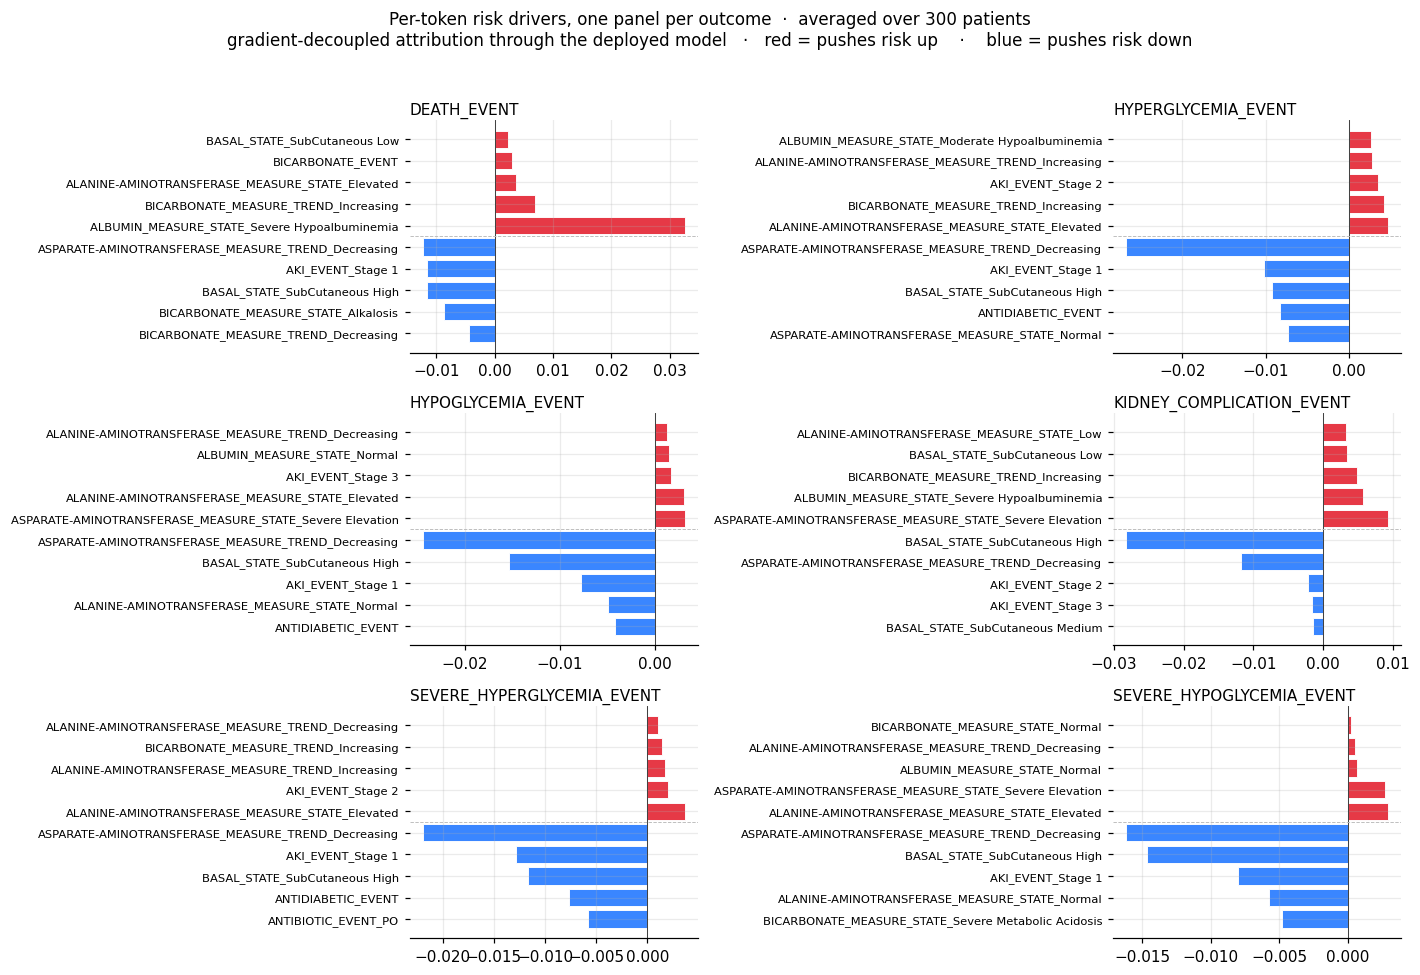
\includegraphics[width=\textwidth]{xai_all_outcomes.png}
  \caption{Per-token top risk drivers for all six forecast outcomes, recovered from INTERVenE-Enc by gradient-decoupled sparse-transcoder attribution and averaged over 300 test patients. Within each panel the bars are signed gradient$\times$activation contributions summed over layers and features; red tokens push the predicted risk up, blue push it down. All drivers are named KBTA concepts (states, trends, and events). x-axis scales are panel-specific, so bar lengths should be compared only within a panel.}
  \label{fig:xai-all}
\end{figure*}